\newlength{\cftchapnumwidth}
\documentclass[essay,paper]{pmk-graduate}

% Класс pmk-graduate.cls используется без изменений.
\usepackage{amsmath,amssymb}
\usepackage{graphicx}
\usepackage{booktabs,tabularx,array,longtable}
\usepackage{enumitem}
\usepackage{listings}
\usepackage{hyperref}
\usepackage{csquotes}
\addbibresource{rup_references.bib}

\hypersetup{colorlinks=true,linkcolor=black,citecolor=black,urlcolor=blue}
\setlist{nosep,leftmargin=1.25cm}
\renewcommand{\arraystretch}{1.2}
\begin{document}
\year{2026-2027}
\subject{Методы проектирования и разработки программного обеспечения}

% Студент
\student{Мартиросянц Александр Евгеньевич
\brief А.\,Е.\,Мартиросянц
\group 47
\english Martirosyants Alexander Evgenievich
}
% Научный руководитель
\superviser{Дадеркин Дмитрий Ольгердович
\brief Д.\,О.\,Дадеркин
\position доцент кафедры информатики
\degree д.\,ф.-м.\,н. % Учёная степень. При отсутствии убрать строку
\rank профессор % Учёное звание. При отсутствии убрать строку
}

\program{ics}
\title{Методология RUP: диаграммы состояний\english RUP methodology: state machine diagrams}
\goal{Исследовать место диаграмм состояний UML в методологии Rational Unified Process, причины возникновения соответствующих подходов, правила построения моделей состояний, практическое применение, преимущества, ограничения и современные направления развития.}

\clearpage

\introduction

Разработка программного обеспечения представляет собой не только написание исходного кода, но и последовательное преобразование потребностей пользователей в требования, архитектурные решения, программные компоненты и проверяемый продукт. По мере роста сложности систем становится недостаточно описывать только состав модулей и связи между ними. Необходимо понимать, как отдельные объекты ведут себя во времени, какие события вызывают изменение их поведения, какие условия ограничивают переходы и какие действия должны выполняться при входе в определённое состояние.

Одним из способов описания такого поведения являются диаграммы состояний языка UML (Unified Modeling Language). В контексте Rational Unified Process (RUP) они используются как средство анализа и проектирования динамического поведения объектов и подсистем. Важно подчеркнуть, что диаграмма состояний не является самостоятельной методологией RUP: это нотация UML, которую RUP включает в набор средств моделирования и применяет в зависимости от задач конкретного проекта.

Актуальность темы обусловлена тем, что программные системы всё чаще управляют процессами, в которых поведение объекта зависит от его текущего состояния: заказ может быть создан, оплачен, отправлен и закрыт; учётная запись может ожидать подтверждения, быть активной или заблокированной; сетевое соединение проходит этапы установления, передачи данных и завершения. Ошибки в таких переходах приводят к некорректным сценариям, нарушению бизнес-правил и сложностям тестирования. Явная модель состояний позволяет выявить подобные проблемы ещё до реализации.

Исторический аспект темы также важен. RUP появился в условиях, когда крупные программные проекты испытывали трудности из-за разрозненных процессов разработки, позднего обнаружения ошибок и отсутствия общего языка общения между аналитиками, архитекторами, программистами и заказчиками. Одновременно развивались объектно-ориентированные методы и UML, позволявший унифицировать представление структуры и поведения систем. RUP объединил итерационный процесс, архитектурный подход, управление требованиями и практики моделирования.

Цель работы — исследовать место диаграмм состояний UML в RUP и показать, каким образом моделирование состояний помогает проектировать, проверять и сопровождать программные системы.

Для достижения цели поставлены следующие задачи:
\begin{enumerate}
  \item рассмотреть исторические и технологические предпосылки возникновения RUP и UML;
  \item раскрыть назначение RUP, его принципы, фазы и дисциплины;
  \item определить роль диаграмм состояний в UML и в рабочих процессах RUP;
  \item изучить основные элементы диаграмм состояний и правила их построения;
  \item разработать пример модели состояний для объекта программной системы;
  \item оценить преимущества и ограничения применения диаграмм состояний;
  \item объяснить, какие подходы используются сегодня и почему RUP применяется иначе, чем в период своего наибольшего распространения.
\end{enumerate}

Объект исследования — процесс проектирования и разработки программного обеспечения в рамках RUP. Предмет исследования — диаграммы состояний UML как средство моделирования динамического поведения системы. В работе применяются историко-аналитический метод, сравнительный анализ, формализация примера и обобщение практических рекомендаций.

\section{Исторические предпосылки появления RUP и UML}

\subsection{Проблемы разработки программного обеспечения до появления RUP}

В 1970–1980-е годы программные системы становились всё более масштабными. Компьютеры начали использоваться не только для научных расчётов и отдельных инженерных задач, но и для управления производством, финансовыми операциями, документооборотом и корпоративными процессами. Увеличивались объём кода, число участников проекта, количество внешних интерфейсов и требования к надёжности.

Традиционные последовательные схемы разработки предполагали, что требования можно полностью определить в начале проекта, после чего последовательно выполнить анализ, проектирование, программирование, тестирование и внедрение. На практике требования менялись, а ошибки анализа обнаруживались уже после того, как на их основе создавались архитектура и программные компоненты. Чем позже обнаруживалась ошибка, тем дороже обходилось её исправление: требовалось пересматривать документацию, код, тесты и интеграционные решения.

Дополнительной проблемой было отсутствие единого способа описания системы. Разные специалисты могли использовать собственные обозначения для одних и тех же понятий. Аналитик описывал сценарии текстом, архитектор рисовал схемы модулей, программист объяснял поведение через код, а тестировщик создавал набор случаев проверки. Связь между этими материалами оказывалась неполной. Это затрудняло проверку полноты требований и передачу проекта между командами.

Объектно-ориентированные методы частично решили проблему, предложив рассматривать систему как совокупность взаимодействующих объектов, обладающих данными и поведением. Однако в первой половине 1990-х годов существовало несколько конкурирующих методов и нотаций. Это приводило к несовместимости моделей и повышало затраты на обучение и использование CASE-средств. Возникла потребность в едином языке моделирования и в более управляемом процессе разработки.

\subsection{Формирование UML}

Разработка UML началась в Rational Software Corporation в 1994 году, когда Грэди Буч и Джеймс Рамбо приступили к объединению своих объектно-ориентированных методов. В 1995 году к работе присоединился Ивар Якобсон со своей методикой OOSE и опытом использования вариантов применения (use cases). Эти специалисты стали известны как «три амиго». Их задачей было не просто создать новый графический язык, а объединить лучшие идеи существовавших методов и обеспечить единый способ описания программных систем \cite{omgwhyuml}.

В 1997 году Object Management Group (OMG) приняла UML 1.1 в качестве стандарта. Впоследствии язык развивался; значимая версия UML 2.0 была принята в 2005 году, а спецификация UML 2.5.1 опубликована в декабре 2017 года \cite{omguml}. Стандартизация позволила разработчикам инструментов, учебных материалов и проектных методик опираться на согласованную семантику элементов диаграмм.

Отдельное влияние на развитие диаграмм состояний оказали работы Дэвида Харела. В 1987 году он предложил Statecharts — визуальный формализм, расширяющий классические конечные автоматы и позволяющий описывать иерархические и параллельные состояния. Эти идеи помогли сделать модели поведения пригодными для более сложных реактивных систем. UML использует близкие концепции в своей модели автоматов состояний \cite{harel1987}.

UML включает структурные диаграммы, описывающие статическую организацию системы, и диаграммы поведения, показывающие её динамику. К структурным относятся, например, диаграммы классов и компонентов. К поведенческим — диаграммы вариантов использования, деятельности, последовательности, коммуникации и состояний. Выбор конкретной диаграммы зависит от вопроса, на который должна ответить модель.

\subsection{Истоки и развитие Rational Unified Process}

RUP сформировался в Rational в 1990-е годы как обобщение практик разработки сложных объектно-ориентированных систем. Важное влияние оказали метод Objectory, идеи разработки на основе вариантов использования, архитектурно-центрированный подход и итерационная организация работ. В конце 1990-х годов RUP оформился как коммерчески распространяемый процесс, сопровождавшийся описаниями ролей, действий, артефактов и рекомендаций \cite{kruchten2003,jacobson1999}.

В 2003 году IBM приобрела Rational Software. RUP вошёл в семейство средств IBM Rational и продолжил использоваться как настраиваемая процессная база. Позднее акцент отрасли сместился к гибким методам, непрерывной интеграции, DevOps и облачной разработке. Это не означает, что идеи RUP исчезли: итеративность, архитектурное управление, управление требованиями и проверка качества продолжают применяться, но всё чаще в более лёгких и адаптированных процессах.

\subsection{Почему потребовалась отдельная модель поведения}

Структурная модель показывает, какие классы существуют и как они связаны, но не всегда объясняет, какие действия разрешены объекту в конкретный момент. Например, наличие класса «Заказ» и атрибутов «номер», «дата» и «сумма» ничего не говорит о том, допустимо ли отменить заказ после отправки или можно ли повторно выполнить оплату.

Текстовое описание поведения может содержать исключения и условия, но при увеличении числа сценариев становится трудно проверить его полноту. Диаграмма состояний решает эту задачу за счёт явного перечисления допустимых состояний и переходов. Она особенно полезна для объектов с жизненным циклом, протоколов взаимодействия, интерфейсов устройств, процессов обработки заявок и других систем, где реакция на событие зависит от текущего состояния \cite{harel1987,fowler2003}.

\section{Методология Rational Unified Process}

\subsection{Понятие и назначение RUP}

Rational Unified Process — это итерационная и инкрементальная методология (точнее, настраиваемый процесс разработки), предназначенная для организации полного жизненного цикла программного проекта. RUP описывает, кто выполняет работу, какие действия осуществляются, какие артефакты создаются и какие результаты должны быть получены. Он не задаёт единственный неизменный сценарий: процесс адаптируется под масштаб проекта, требования к качеству, состав команды и ограничения предметной области \cite{kruchten2003,jacobson1999}.

В основе RUP лежат несколько взаимосвязанных принципов:
\begin{itemize}
  \item \textbf{итерационная разработка} — система создаётся серией управляемых циклов, каждый из которых даёт проверяемый результат;
  \item \textbf{управление требованиями} — требования фиксируются, уточняются и связываются с проектными решениями и тестами;
  \item \textbf{архитектурная основа} — ключевые архитектурные решения принимаются и проверяются на ранних этапах;
  \item \textbf{моделирование} — сложные аспекты системы представляются в виде моделей, пригодных для анализа и обсуждения;
  \item \textbf{непрерывная проверка качества} — тестирование и оценка результатов проводятся на протяжении проекта;
  \item \textbf{контроль изменений} — изменения требований, моделей и кода отслеживаются и управляются.
\end{itemize}

RUP отличается от простого перечня фаз тем, что разделяет жизненный цикл проекта и дисциплины работ. Фазы показывают, на каком этапе находится проект и какие контрольные результаты должны быть достигнуты. Дисциплины описывают виды деятельности, которые могут выполняться в разных фазах с различной интенсивностью.

\subsection{Фазы жизненного цикла}

Жизненный цикл RUP включает четыре фазы.

\textbf{Начало (Inception).} Определяются границы проекта, основные заинтересованные стороны, бизнес-цели, ключевые варианты использования, ограничения и предварительная оценка рисков. На этой фазе важно понять, имеет ли смысл продолжать проект и достаточно ли согласовано его назначение. Детальная модель состояний всех объектов обычно не требуется, однако могут быть выявлены критические жизненные циклы, требующие дальнейшего анализа.

\textbf{Уточнение (Elaboration).} Прорабатываются требования, проверяются архитектурные решения, уточняются наиболее рискованные сценарии и создаётся архитектурная основа системы. Именно здесь часто строятся подробные диаграммы состояний для критичных объектов и подсистем. Модели помогают проверить, что архитектура поддерживает необходимые режимы работы и исключительные ситуации.

\textbf{Конструирование (Construction).} Создаётся основная часть продукта. Модели уточняются по мере реализации, используются при разработке кода и тестов. Не каждая диаграмма должна быть детализирована до уровня каждой строки программы: модель поддерживается настолько подробно, насколько это помогает разработке и проверке.

\textbf{Внедрение (Transition).} Система передаётся пользователям, выполняются приёмочные проверки, обучение, миграция данных и исправление обнаруженных проблем. Диаграммы состояний могут использоваться при подготовке эксплуатационной документации, сценариев поддержки и тестов на корректность переходов.

\begin{table}[ht]
\centering
\caption{Фазы RUP и возможное использование диаграмм состояний}
\begin{tabularx}{\textwidth}{|p{2.8cm}|X|X|}
\hline
\textbf{Фаза} & \textbf{Основной результат} & \textbf{Роль модели состояний} \\ \hline
Начало & Видение, границы и основные риски & Выявление объектов со сложным жизненным циклом \\ \hline
Уточнение & Проверенная архитектурная основа & Формализация критичных состояний, событий и ограничений \\ \hline
Конструирование & Реализованные компоненты и тесты & Уточнение поведения и создание проверок переходов \\ \hline
Внедрение & Готовый к эксплуатации продукт & Поддержка приёмочных сценариев и документации \\ \hline
\end{tabularx}
\end{table}

\subsection{Дисциплины RUP и место моделирования}

К основным инженерным дисциплинам RUP относятся моделирование бизнеса, определение требований, анализ и проектирование, реализация, тестирование и развёртывание. Управляющие дисциплины включают управление конфигурацией и изменениями, управление проектом и обеспечение среды разработки. Их интенсивность меняется в зависимости от фазы.

Диаграммы состояний относятся прежде всего к анализу и проектированию. При анализе они помогают понять предметную область и уточнить правила поведения. При проектировании — описать поведение программного объекта, компонента или подсистемы. В тестировании диаграмма может стать источником сценариев: для каждого перехода проверяются событие, условие, ожидаемое состояние и возможные альтернативы.

Следует избегать ошибочного представления, будто RUP требует строить все возможные диаграммы UML для каждого проекта. Смысл процессного подхода — выбирать артефакты по ценности. Если объект имеет два простых состояния и один очевидный переход, отдельная диаграмма может быть избыточна. Если же объект обладает десятками состояний, параллельными режимами и множеством исключений, модель становится полезным средством контроля сложности.

\subsection{Роли и артефакты}

В RUP распределяются роли аналитика, архитектора, проектировщика, разработчика, тестировщика, руководителя проекта и других участников. Один человек в небольшой команде может совмещать несколько ролей. Диаграмму состояний может подготовить системный аналитик совместно с экспертом предметной области, а затем уточнить архитектор и разработчик.

Артефактами, связанными с моделированием поведения, могут быть модель анализа и проектирования, описание вариантов использования, спецификации требований, проектные классы, тестовые сценарии и результаты проверок. Важно поддерживать трассируемость: каждое существенное состояние или ограничение должно быть связано с требованием, а каждый критичный переход — с проверкой.

\section{Диаграммы состояний UML: понятия и элементы}

\subsection{Назначение диаграммы состояний}

Диаграмма состояний (state machine diagram) описывает поведение отдельного объекта или системы как реакцию на события. Модель состоит из состояний, переходов между ними, событий-триггеров, условий-ограничений и действий. В каждый момент объект находится в некотором активном состоянии или наборе вложенных состояний, а поступление события может привести к изменению конфигурации состояний \cite{omguml}.

В простейшем случае диаграмма похожа на ориентированный граф: вершины соответствуют состояниям, а дуги — переходам. Однако UML определяет более богатую семантику: составные состояния, вложенность, ортогональные области, псевдосостояния, действия при входе и выходе, внутренние переходы и историю состояния.

Диаграмма отвечает на вопросы: какие режимы работы возможны; какие события допускаются в каждом режиме; какие условия должны быть выполнены; какие действия происходят при переходе; какие состояния являются начальными и конечными; какие сценарии запрещены.

\subsection{Состояние}

Состояние — это ситуация в жизненном цикле объекта, в которой выполняется некоторое условие, объект ожидает событие или выполняет деятельность. На диаграмме UML простое состояние изображается прямоугольником со скруглёнными углами. Внутри указывается его имя. При необходимости в состоянии могут быть заданы действия входа (entry), выхода (exit) и выполняемая деятельность (do).

Например, заказ интернет-магазина может находиться в состояниях «Создан», «Ожидает оплаты», «Оплачен», «Собирается», «Отправлен», «Доставлен» и «Отменён». Каждое состояние должно иметь однозначный смысл с точки зрения предметной области. Не рекомендуется создавать состояния, которые обозначают лишь технические детали реализации и не влияют на допустимое поведение.

\subsection{Переход и его запись}

Переход задаёт допустимое перемещение из исходного состояния в целевое. Типовая запись имеет вид:
\[
  \text{событие} \; [\text{условие}] \; / \; \text{действие}.
\]

Событие запускает проверку перехода; условие (guard) должно быть истинным, чтобы переход мог выполниться; действие (effect) выполняется в ходе перехода. Например, запись \texttt{оплатаПолучена [сумма = итого] / зафиксироватьПлатёж()} означает, что переход разрешён при получении события об оплате и совпадении суммы с суммой заказа.

Условие не является действием: оно только определяет возможность перехода. Действие, напротив, изменяет данные или вызывает операцию. Смешение этих понятий приводит к неясной модели и затрудняет тестирование.

\subsection{Начальное и конечное псевдосостояния}

Начальное псевдосостояние изображается закрашенным кружком и показывает точку входа в автомат. От него обычно исходит переход к начальному рабочему состоянию. Конечное состояние изображается в виде закрашенного кружка внутри окружности. Оно обозначает завершение соответствующего поведения. Конечное состояние не следует путать с обычным состоянием «Закрыт»: первое завершает выполнение автомата или региона, второе может оставаться полноценным состоянием объекта.

\subsection{События, сигналы и временные триггеры}

Событие — это факт, на который автомат может реагировать. В UML применяются события вызова операции, сигнальные события, временные события и события изменения условия. В прикладной системе это могут быть действия пользователя, сообщения от внешнего сервиса, истечение срока ожидания или изменение значения атрибута.

При проектировании важно определить источник события и правила его обработки. Например, событие «оплата получена» должно поступать от надёжного платёжного компонента, а не генерироваться произвольно пользовательским интерфейсом. Если событие может прийти повторно, модель должна определять, является ли повторная обработка допустимой, игнорируемой или ошибочной.

\subsection{Действия entry, exit и do}

Действие \texttt{entry} выполняется при входе в состояние, \texttt{exit} — при выходе, а \texttt{do} обозначает деятельность, которая продолжается во время нахождения в состоянии и может быть прервана переходом. Например, при входе в состояние «Ожидает оплаты» запускается таймер; во время состояния система ожидает подтверждение; при выходе таймер отменяется.

Эти действия позволяют показать важные эффекты, не перегружая диаграмму низкоуровневыми деталями. В то же время бизнес-правила и алгоритмы, которые сами по себе сложны, лучше описывать отдельными спецификациями или диаграммами деятельности.

\subsection{Составные состояния и ортогональные регионы}

Составное состояние объединяет вложенные состояния и позволяет группировать поведение. Например, состояние «Обрабатывается» может включать «Проверяется», «Комплектуется» и «Передаётся в доставку». Это уменьшает число пересекающихся линий и помогает управлять сложностью.

Ортогональные регионы показывают параллельные аспекты поведения. Например, в системе управления устройством отдельно могут моделироваться режим питания и режим связи. Оба региона активны одновременно, но описывают разные измерения состояния. Параллелизм следует вводить только тогда, когда он отражает реальную независимость процессов; иначе модель становится сложнее для понимания.

\subsection{Исторические псевдосостояния и внутренние переходы}

Исторические псевдосостояния позволяют при повторном входе в составное состояние восстановить ранее активное вложенное состояние. Это полезно, если временное прерывание процесса не должно приводить к возврату к самому началу. Внутренний переход обрабатывает событие без выхода из текущего состояния, поэтому действия выхода и повторного входа не выполняются.

Подобные конструкции особенно важны для сложных автоматов, но их следует использовать осознанно. Если диаграмма содержит много исторических переходов и вложенных уровней, полезно дополнить её текстовым описанием семантики и набором тестов.

\section{Построение диаграмм состояний в рамках RUP}

\subsection{От требования к модели поведения}

Работа над диаграммой начинается не с рисования фигур, а с анализа требований и предметной области. Сначала выделяется объект, жизненный цикл которого необходимо описать. Затем из требований, сценариев использования, регламентов и интервью с экспертами извлекаются возможные состояния, события и ограничения.

Практический порядок действий может быть следующим:
\begin{enumerate}
  \item выбрать объект моделирования и сформулировать границы его ответственности;
  \item определить начальное состояние и условия завершения жизненного цикла;
  \item перечислить устойчивые состояния, различающиеся допустимым поведением;
  \item определить события, которые могут поступать в каждом состоянии;
  \item задать условия переходов и действия, сопровождающие переход;
  \item проверить, что нет недостижимых состояний и переходов без смысла;
  \item проанализировать альтернативные и ошибочные сценарии;
  \item связать переходы с требованиями и тестами;
  \item уточнить модель в следующей итерации RUP после получения обратной связи.
\end{enumerate}

Такой порядок соответствует итерационной природе RUP. На раннем этапе модель может быть укрупнённой и содержать только основные режимы. После проверки архитектурных рисков она детализируется: добавляются таймеры, повторные события, исключения и условия, связанные с внешними сервисами.

\subsection{Выбор объекта моделирования}

Не каждый класс требует диаграммы состояний. Хорошими кандидатами являются объекты, для которых допустимые операции зависят от текущего статуса. Примеры: заказ, платёж, заявка, сессия пользователя, сетевое соединение, задача планировщика, устройство с несколькими режимами работы.

Плохим кандидатом может быть простой справочник или объект-значение, который не имеет самостоятельного жизненного цикла. Если объект содержит только набор полей и не меняет поведение в зависимости от истории, диаграмма может не дать дополнительной пользы.

Граница автомата должна быть согласована с ответственностью объекта. Если диаграмма пытается описать сразу весь интернет-магазин, платёжную систему, службу доставки и интерфейс пользователя, она становится чрезмерно большой. Лучше разделить поведение на несколько автоматов и описать взаимодействие между ними через события и контракты.

\subsection{Проверка полноты и непротиворечивости}

При проверке модели задаются вопросы: существует ли начальное состояние; достижимо ли каждое важное состояние; может ли объект попасть в тупик; не допускается ли переход, противоречащий бизнес-правилам; обрабатываются ли повторные и запоздавшие события; определено ли поведение при ошибке внешней системы; не возникает ли неоднозначность, когда одновременно подходят несколько переходов.

Важным приёмом является построение таблицы переходов. Для каждого состояния перечисляются события, условия, целевое состояние и действие. Таблица помогает заметить пропущенные случаи и может использоваться при создании тестов.

\begin{table}[ht]
\centering
\caption{Фрагмент таблицы переходов для заказа}
\small
\begin{tabularx}{\textwidth}{|p{2.4cm}|p{2.6cm}|X|p{2.5cm}|}
\hline
\textbf{Исходное состояние} & \textbf{Событие} & \textbf{Условие} & \textbf{Результат} \\ \hline
Создан & Подтвердить & Данные корректны & Ожидает оплаты \\ \hline
Ожидает оплаты & Оплата получена & Сумма совпадает & Оплачен \\ \hline
Ожидает оплаты & Истёк срок & Оплата не поступила & Отменён \\ \hline
Оплачен & Передать в сборку & Товары доступны & Собирается \\ \hline
Собирается & Передать перевозчику & Комплектация завершена & Отправлен \\ \hline
Отправлен & Подтверждение доставки & Доставка подтверждена & Доставлен \\ \hline
\end{tabularx}
\normalsize
\end{table}

\subsection{Связь с другими диаграммами UML}

Диаграмма состояний не заменяет остальные виды моделей. Диаграмма вариантов использования показывает цели и взаимодействия акторов с системой. Диаграмма последовательности раскрывает обмен сообщениями в конкретном сценарии. Диаграмма деятельности описывает поток работ и ветвления. Диаграмма классов фиксирует структуру объектов и их отношения. Диаграмма состояний отвечает за допустимое поведение объекта в течение жизненного цикла.

В RUP эти модели могут уточнять друг друга. Вариант использования «Оформить заказ» задаёт основной сценарий. Диаграмма последовательности показывает вызовы между интерфейсом, сервисом заказа и платёжным шлюзом. Диаграмма состояний фиксирует, что заказ может перейти из «Ожидает оплаты» в «Оплачен» только после подтверждения платежа. Диаграмма классов показывает, где хранится статус и какие операции доступны объекту.

\section{Практический пример: жизненный цикл заказа интернет-магазина}

\subsection{Постановка задачи}

Рассмотрим упрощённую систему интернет-магазина. Пользователь формирует заказ, система проверяет корректность данных и доступность товаров, затем ожидает оплату. После подтверждения платежа заказ передаётся на сборку, далее — перевозчику и завершается после подтверждения доставки. Если пользователь не оплатил заказ в установленный срок, заказ отменяется. После передачи заказа перевозчику обычная отмена уже невозможна и должна обрабатываться отдельной процедурой возврата.

Цель модели — описать жизненный цикл объекта «Заказ», исключить недопустимые переходы и обеспечить тестируемость бизнес-правил. В примере не рассматриваются все реальные детали логистики, возвратов, частичных оплат и складского резервирования: модель намеренно ограничена основным сценарием.

\subsection{Определение состояний}

Выделим следующие состояния: «Создан», «Ожидает оплаты», «Оплачен», «Собирается», «Отправлен», «Доставлен» и «Отменён». Первое является начальным рабочим состоянием, «Доставлен» и «Отменён» — терминальными бизнес-состояниями заказа. При этом в UML их можно представить как обычные именованные состояния, из которых при необходимости переходят к конечному псевдосостоянию автомата.

Состояние «Ожидает оплаты» означает, что заказ прошёл базовую проверку и ожидает подтверждение платёжного сервиса. Состояние «Оплачен» фиксирует подтверждённый платёж. «Собирается» означает, что склад комплектует заказ. «Отправлен» означает, что перевозчик принял отправление. «Доставлен» фиксирует завершение основного цикла.

\subsection{Диаграмма состояний}

На рисунке 1 приведена упрощённая диаграмма. Она показывает только основные переходы, не раскрывая внутреннее устройство платёжного и логистического сервисов.

\begin{figure}[ht]
\centering
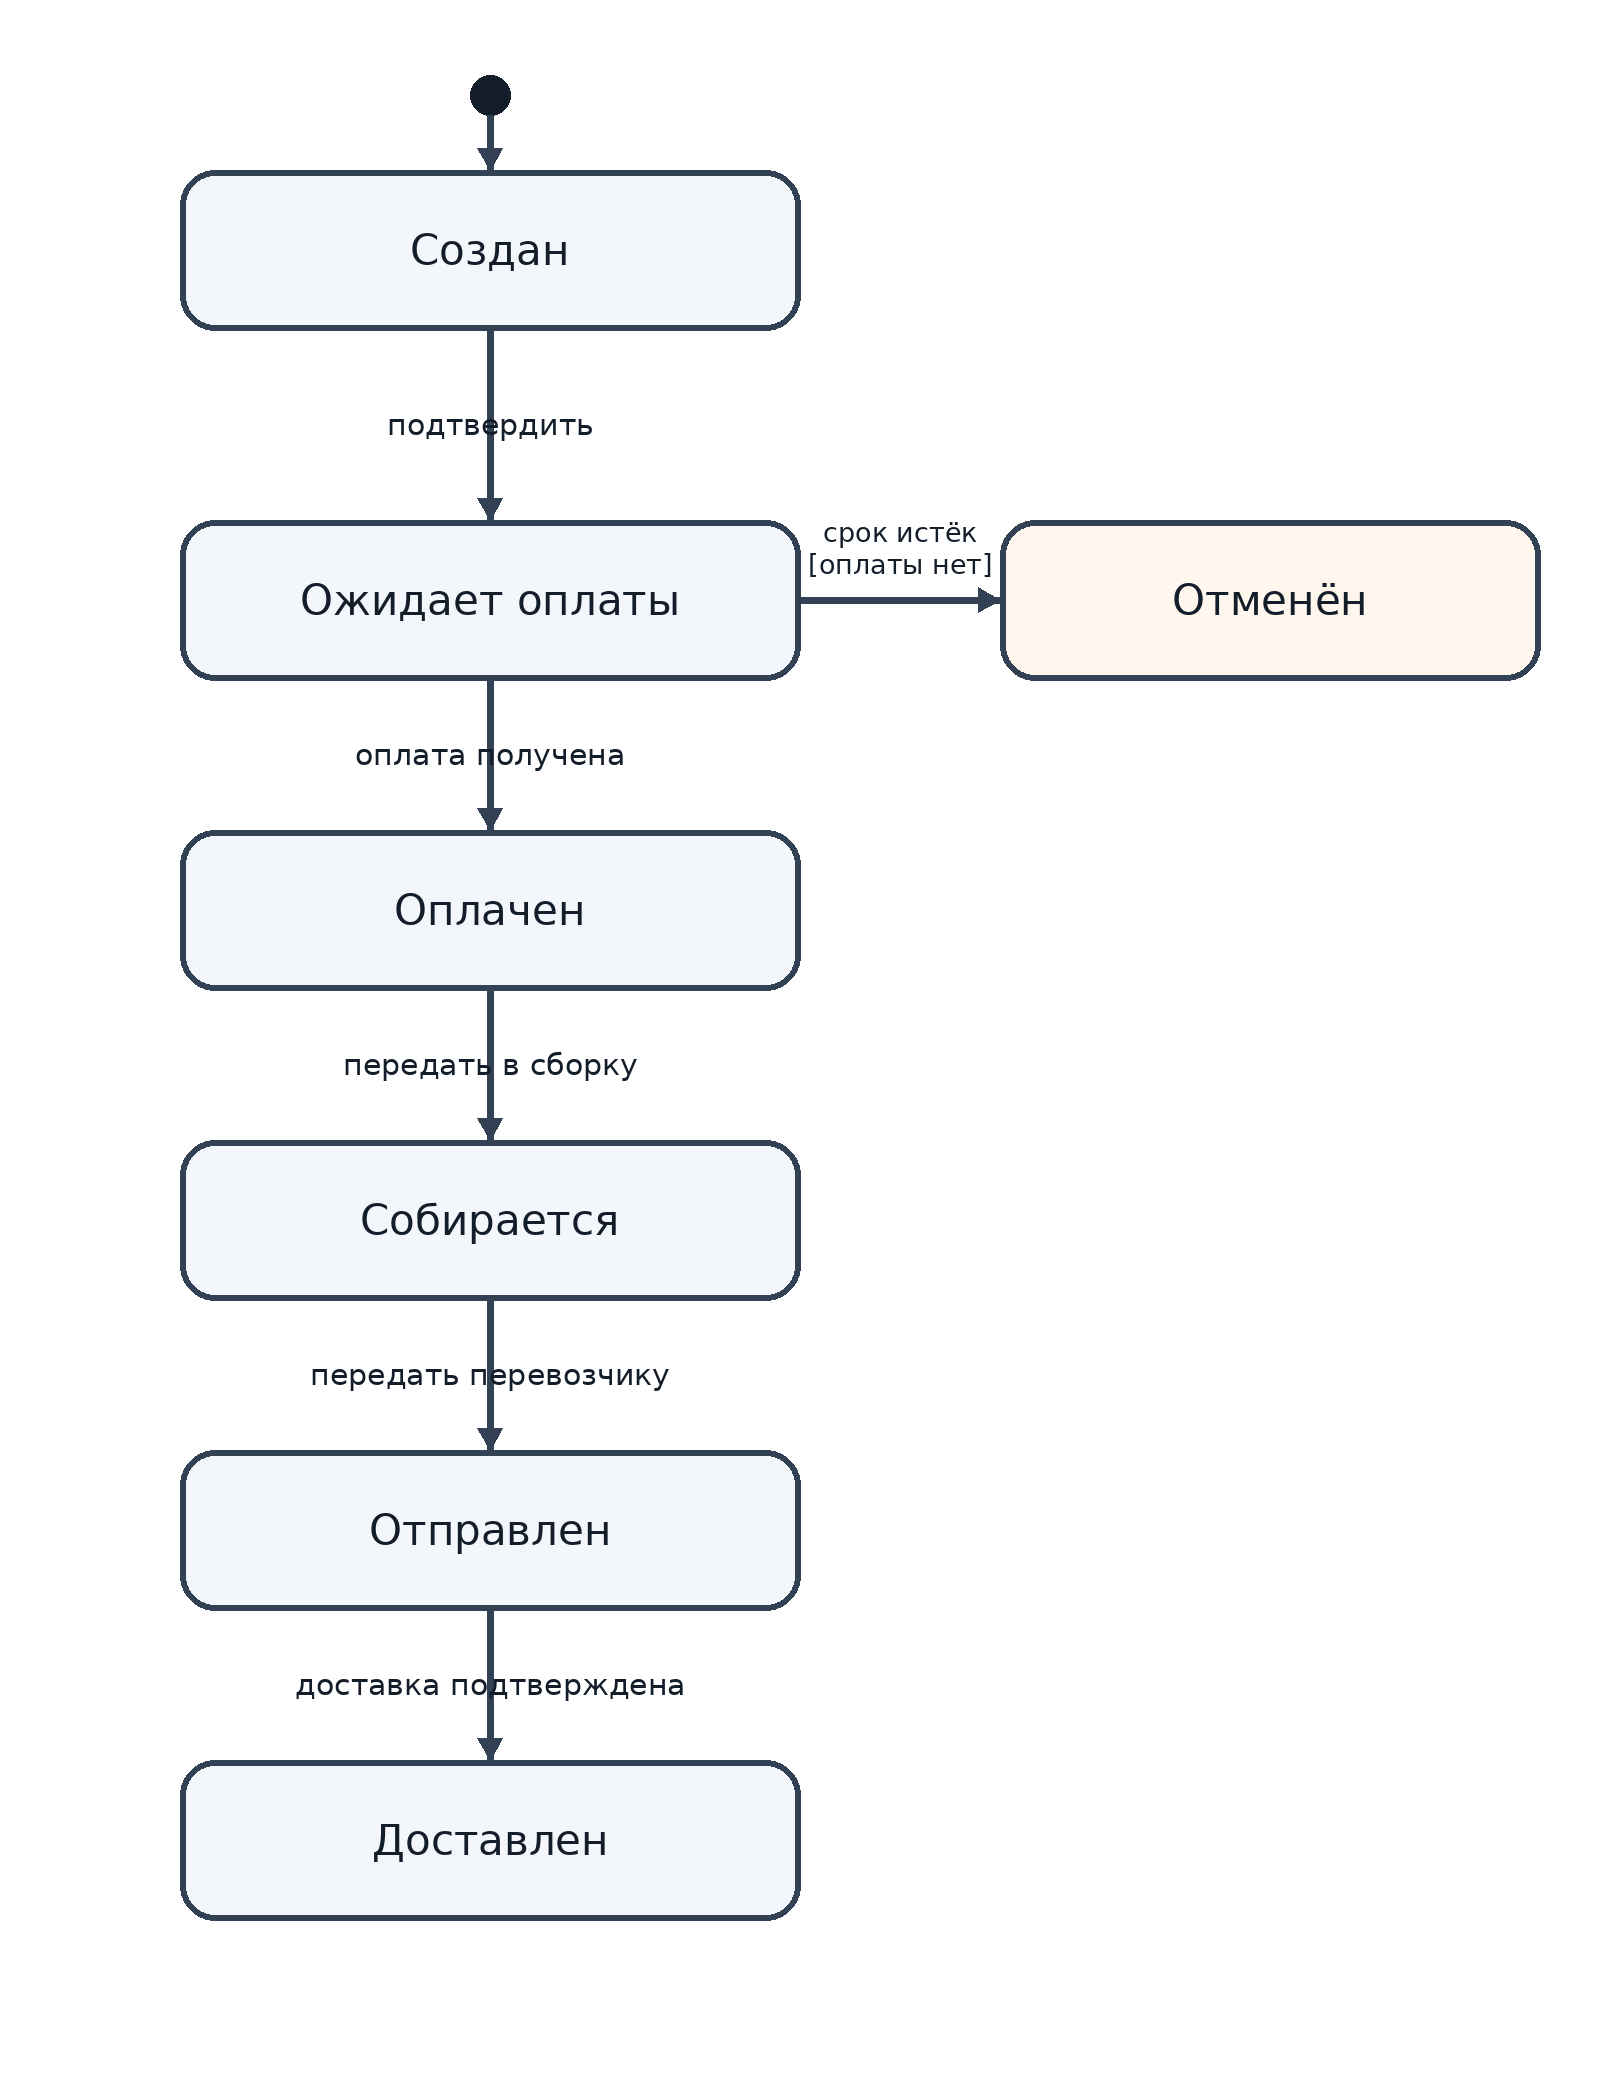
\includegraphics[width=0.65\textwidth]{order_states.png}
\caption{Упрощённая диаграмма состояний объекта «Заказ»}
\end{figure}

\subsection{Условия и действия переходов}

Переход из «Создан» в «Ожидает оплаты» разрешается после проверки состава заказа и контактных данных. При входе в «Ожидает оплаты» система резервирует товары на ограниченное время и запускает таймер ожидания. Переход в «Оплачен» выполняется только при получении подтверждения от платёжного сервиса и совпадении суммы с итоговой стоимостью заказа.

Если время ожидания истекло, а платёж не поступил, заказ переходит в «Отменён», резерв снимается, а пользователю отправляется уведомление. При поступлении запоздавшего подтверждения оплаты система не должна автоматически возвращать отменённый заказ в активный процесс. Такое событие следует обработать отдельным правилом: например, инициировать возврат средств или передать ситуацию оператору.

После перехода в «Оплачен» заказ передаётся на сборку. Событие «Передать в сборку» допустимо, если товары доступны и резерв подтверждён. После завершения комплектации заказ передаётся перевозчику. После подтверждения доставки заказ переходит в конечное бизнес-состояние «Доставлен».

\subsection{Таблица проверок для тестирования}

Из диаграммы можно получить тестовые сценарии. Для каждого перехода проверяется нормальный случай, нарушение условия, повтор события и попытка выполнить недопустимую операцию. Например, тест должен подтвердить, что заказ в состоянии «Ожидает оплаты» не переходит в «Оплачен» без валидного подтверждения. Отдельно проверяется, что заказ в состоянии «Отправлен» не может быть отменён стандартной командой отмены.

\begin{table}[ht]
\centering
\caption{Примеры тестов на основе диаграммы состояний}
\begin{tabularx}{\textwidth}{|p{3.1cm}|X|X|}
\hline
\textbf{Тест} & \textbf{Действие} & \textbf{Ожидаемый результат} \\ \hline
T1 & Подтвердить корректный созданный заказ & Состояние меняется на «Ожидает оплаты» \\ \hline
T2 & Получить подтверждение оплаты на верную сумму & Состояние меняется на «Оплачен» \\ \hline
T3 & Получить подтверждение с неверной суммой & Переход не выполняется, фиксируется ошибка \\ \hline
T4 & Дождаться истечения срока без оплаты & Заказ переходит в «Отменён», резерв снимается \\ \hline
T5 & Повторно отправить событие оплаты после перехода в «Оплачен» & Повтор не создаёт второй платёж и не нарушает состояние \\ \hline
T6 & Попытаться отменить отправленный заказ & Обычная отмена отклоняется; запускается отдельный процесс возврата \\ \hline
\end{tabularx}
\end{table}

\subsection{Как пример вписывается в RUP}

На фазе начала проекта команда выявляет, что заказ имеет сложный жизненный цикл, а ошибки переходов связаны с финансовыми и операционными рисками. На фазе уточнения аналитик и архитектор формализуют состояния, события и ограничения, после чего проверяют архитектурные решения для обработки платежей и таймеров. На фазе конструирования разработчики реализуют логику переходов, а тестировщики используют модель для построения тестов. На фазе внедрения диаграмма помогает объяснить поведение системы специалистам сопровождения.

Пример показывает ключевую ценность модели: она связывает бизнес-правило с программной реализацией и проверкой. Диаграмма не заменяет код и не гарантирует отсутствие ошибок сама по себе, но делает правила явными и облегчает обсуждение неоднозначных ситуаций.

\section{Преимущества и недостатки диаграмм состояний}

\subsection{Преимущества}

\begin{enumerate}
  \item \textbf{Наглядность жизненного цикла.} Все основные режимы объекта представлены в единой модели, поэтому участникам проекта легче понять, где находится объект и какие изменения допустимы.
  \item \textbf{Формализация бизнес-правил.} Условия переходов делают явными ограничения, которые в текстовом описании могут быть не замечены.
  \item \textbf{Раннее выявление противоречий.} Недостижимые состояния, отсутствующие переходы и неоднозначные сценарии можно обнаружить до завершения реализации.
  \item \textbf{Поддержка тестирования.} Переходы и состояния дают основу для тестов состояний, переходов, граничных случаев и обработки повторных событий.
  \item \textbf{Улучшение коммуникации.} Диаграмму могут обсуждать аналитики, разработчики, тестировщики и эксперты предметной области.
  \item \textbf{Поддержка сопровождения.} При изменении требований модель помогает определить, какие части поведения затронуты и какие проверки необходимо обновить.
  \item \textbf{Масштабирование через вложенность.} Составные состояния и регионы позволяют структурировать сложное поведение без обязательного сведения всех деталей в одну плоскую схему.
\end{enumerate}

\subsection{Недостатки и ограничения}

\begin{enumerate}
  \item \textbf{Риск чрезмерной детализации.} Если моделировать каждое техническое событие и каждую временную переменную, диаграмма становится громоздкой и теряет обзорность.
  \item \textbf{Сложность для неспециалистов.} Составные состояния, история и ортогональные регионы требуют знания UML и могут быть трудны для чтения без пояснений.
  \item \textbf{Проблема синхронизации с кодом.} Если диаграмма не обновляется после изменения реализации, она превращается в устаревшую документацию.
  \item \textbf{Неполнота при изолированном использовании.} Диаграмма не описывает полностью алгоритмы, структуру данных, интерфейсы и последовательность взаимодействия компонентов.
  \item \textbf{Неоднозначность требований.} UML задаёт семантику элементов, но не может самостоятельно устранить неясные или противоречивые требования заказчика.
  \item \textbf{Ограниченная ценность для простых объектов.} Для объектов без сложного поведения диаграмма может оказаться лишним артефактом.
\end{enumerate}

\subsection{Сравнение с текстовым описанием}

Текстовое описание удобно для пояснения мотивации и бизнес-контекста, но его сложнее проверять на полноту. Диаграмма лучше показывает структуру переходов, однако не всегда способна вместить все детали. Наиболее эффективен комбинированный вариант: диаграмма задаёт карту поведения, а таблица или текст уточняет условия, побочные эффекты и исключения.

\begin{table}[ht]
\centering
\caption{Сравнение способов описания поведения}
\begin{tabularx}{\textwidth}{|p{3cm}|X|X|}
\hline
\textbf{Критерий} & \textbf{Текст} & \textbf{Диаграмма состояний} \\ \hline
Читаемость общего потока & Хорошая для короткого сценария & Хорошая для обзора жизненного цикла \\ \hline
Формализация переходов & Зависит от стиля документа & Явно представлены вершинами и дугами \\ \hline
Проверка полноты & Требует внимательного анализа текста & Видны тупики и пропущенные связи \\ \hline
Описание сложных алгоритмов & Подходит для подробных пояснений & Лучше выносить алгоритмы в другие модели \\ \hline
Поддержка тестирования & Нужна дополнительная интерпретация & Переходы непосредственно подсказывают тесты \\ \hline
\end{tabularx}
\end{table}

\section{Современное состояние и развитие подходов}

\subsection{Используется ли RUP сегодня}

RUP не следует рассматривать как универсальный обязательный процесс для всех современных команд. Его полная процессная модель может оказаться слишком тяжёлой для небольшого продукта или команды, работающей короткими циклами. Исследования внедрения RUP отмечали, что адаптация комплексного процесса к конкретной организации сама по себе является непростой задачей, а отрасль постепенно смещалась в сторону более лёгких и гибко настраиваемых процессов \cite{hanssen2007}. При этом отдельные практики RUP могут сохранять ценность в крупных проектах, где важны управление рисками, архитектура и прослеживаемость требований.

Причины изменения распространённости RUP связаны не с тем, что итерационная разработка или моделирование состояний стали бесполезны. Изменился контекст разработки: широкое распространение получили Agile-подходы, Scrum и Kanban, автоматизированные конвейеры сборки и тестирования, облачная инфраструктура, микросервисные архитектуры и DevOps. Командам часто требуется более лёгкий процесс, позволяющий быстро получать обратную связь и непрерывно поставлять изменения.

Поэтому корректнее говорить не о полном исчезновении RUP, а о контекстном использовании его идей. В актуальной документации IBM по управлению проектами по-прежнему описываются фазы и итерации, характерные для RUP, что подтверждает сохранение этих понятий в инструментарии жизненного цикла разработки \cite{ibmphase}. Итеративность, архитектурные прототипы, управление рисками, трассируемость требований и систематическое тестирование остаются полезными практиками.

\subsection{Что пришло на смену и что сохранилось}

На уровне управления командной работой широко применяются Scrum и Kanban. Они не являются прямой заменой UML или RUP: Scrum задаёт рамку организации работы, Kanban — способ визуализации и управления потоком задач. Для инженерной практики используются непрерывная интеграция, автоматизированное тестирование, code review, управление версиями и инфраструктура как код.

На уровне моделирования UML сохраняет значение как стандартизированный язык, но применяется прагматично. Команды могут вести диаграммы в репозиториях, использовать текстовые нотации и генерировать часть моделей из кода. В отдельных областях применяются специализированные формализмы: конечные автоматы, Statecharts, таблицы переходов, протоколы сообщений и модели процессов.

BPMN подходит для описания бизнес-процессов, диаграммы последовательности — для взаимодействия объектов во времени, а диаграммы состояний — для жизненного цикла объекта. Эти средства не следует считать взаимозаменяемыми: каждое решает свой класс задач.

\subsection{Современные инструменты}

Диаграммы состояний могут создаваться в CASE-средствах и UML-редакторах, в том числе в инструментах моделирования общего назначения. Для команды важно не столько название продукта, сколько возможность хранить модель в контролируемом репозитории, просматривать историю изменений, связывать модель с требованиями и тестами и поддерживать совместную работу.

В некоторых проектах диаграмма остаётся документом для анализа и коммуникации. В других — используется как основа для генерации кода или конфигурации. Генерация повышает согласованность модели и реализации, но требует строгого контроля качества модели, ограничений инструмента и результатов генерации. Нельзя считать автоматически созданный код корректным только потому, что исходная диаграмма выглядит логично.

\subsection{Перспективы диаграмм состояний}

С ростом распределённых и событийно-ориентированных систем становится важнее явно описывать состояния, события, тайм-ауты и повторную обработку сообщений. Микросервисы обмениваются сообщениями, которые могут приходить с задержкой или повторно. Состояние процесса часто хранится между запросами, поэтому ошибки переходов способны приводить к дублированию операций или потере согласованности.

Диаграммы состояний помогают обсуждать такие сценарии, но должны дополняться архитектурными решениями: идемпотентностью операций, обработкой ошибок, журналированием, контролем версий событий и проверками целостности. Модель не заменяет эти механизмы, а позволяет заранее определить, какие ситуации система обязана корректно обрабатывать.

\section{Практические рекомендации по применению}

Для эффективного использования диаграмм состояний в проекте рекомендуется придерживаться следующих правил.

\begin{enumerate}
  \item Моделировать поведение конкретного объекта или ограниченной подсистемы, а не пытаться поместить всю систему в одну схему.
  \item Давать состояниям предметные названия, отражающие устойчивый режим объекта.
  \item Формулировать события как факты, а не как неопределённые действия вроде «что-то произошло».
  \item Разделять событие, условие и действие перехода.
  \item Учитывать ошибки внешних систем, повторные события, тайм-ауты и запоздавшие сообщения.
  \item Не добавлять псевдосостояния и сложные конструкции UML только ради демонстрации знания нотации.
  \item Поддерживать связь диаграммы с требованиями и тестами.
  \item Пересматривать модель в каждой итерации, если изменяются правила предметной области.
  \item Использовать диаграмму совместно с другими моделями UML и текстовыми спецификациями.
  \item Определять критерий полезности: если модель не помогает принять решение, проверить поведение или объяснить систему, её детализацию следует сократить.
\end{enumerate}

В RUP эти рекомендации согласуются с принципом управляемой итерационной разработки. Модель создаётся не ради отчётности, а как рабочий инструмент, позволяющий уменьшить неопределённость, выявить риски и улучшить качество проектных решений.

\section*{Выводы}
\addcontentsline{toc}{section}{Выводы}

В ходе работы рассмотрены исторические причины появления RUP и UML, назначение диаграмм состояний и особенности их применения в процессе разработки программного обеспечения. Проведённый анализ позволяет сформулировать следующие выводы.

\begin{enumerate}
  \item RUP возник как ответ на проблемы разработки сложных программных систем: рост требований, высокая стоимость позднего исправления ошибок, разобщённость участников и отсутствие согласованного процесса.
  \item UML сформировался в результате объединения объектно-ориентированных методов Booch, OMT и OOSE. Стандартизация нотации позволила использовать общий язык моделирования в разных инструментах и проектах.
  \item Диаграммы состояний являются частью UML, а не отдельной методологией RUP. RUP предоставляет процессную основу, в рамках которой такие диаграммы применяются по необходимости.
  \item Основная функция диаграммы состояний — формальное описание допустимых режимов объекта и переходов, запускаемых событиями и ограниченных условиями.
  \item Диаграммы особенно полезны для объектов с нетривиальным жизненным циклом: заказов, платежей, заявок, сессий, соединений и управляемых устройств.
  \item На фазе уточнения RUP модель может использоваться для проверки архитектурных рисков; на фазе конструирования — для реализации и тестирования; на фазе внедрения — для сопровождения и объяснения поведения.
  \item На примере заказа интернет-магазина показано, что диаграмма помогает обнаруживать недопустимые переходы, обрабатывать тайм-ауты и учитывать повторные события.
  \item К преимуществам относятся наглядность, формализация правил, раннее выявление ошибок, поддержка тестирования и улучшение коммуникации команды.
  \item К недостаткам относятся риск чрезмерной детализации, необходимость знания UML и вероятность расхождения модели с фактической реализацией.
  \item Современная разработка не отказалась от идей RUP полностью. Чаще используются адаптированные процессы, Agile-практики, DevOps и выборочное моделирование.
  \item Диаграммы состояний сохраняют практическую ценность в системах, где реакция на событие зависит от текущего режима объекта, в том числе в распределённых и событийно-ориентированных приложениях.
\end{enumerate}

Таким образом, диаграммы состояний занимают важное место в инструментарии проектирования программного обеспечения. Их эффективность определяется не количеством построенных схем, а тем, насколько точно они отражают правила предметной области, помогают согласовать требования с реализацией и позволяют систематически проверять поведение системы.

\nocite{*}
\printthebibliography

\end{document}
